\batchmode
\documentclass[twoside]{book}

% Packages required by doxygen
\usepackage{fixltx2e}
\usepackage{calc}
\usepackage{doxygen}
\usepackage[export]{adjustbox} % also loads graphicx
\usepackage{graphicx}
\usepackage[utf8]{inputenc}
\usepackage{makeidx}
\usepackage{multicol}
\usepackage{multirow}
\PassOptionsToPackage{warn}{textcomp}
\usepackage{textcomp}
\usepackage[nointegrals]{wasysym}
\usepackage[table]{xcolor}

% Font selection
\usepackage[T1]{fontenc}
\usepackage[scaled=.90]{helvet}
\usepackage{courier}
\usepackage{amssymb}
\usepackage{sectsty}
\renewcommand{\familydefault}{\sfdefault}
\allsectionsfont{%
  \fontseries{bc}\selectfont%
  \color{darkgray}%
}
\renewcommand{\DoxyLabelFont}{%
  \fontseries{bc}\selectfont%
  \color{darkgray}%
}
\newcommand{\+}{\discretionary{\mbox{\scriptsize$\hookleftarrow$}}{}{}}

% Page & text layout
\usepackage{geometry}
\geometry{%
  a4paper,%
  top=2.5cm,%
  bottom=2.5cm,%
  left=2.5cm,%
  right=2.5cm%
}
\tolerance=750
\hfuzz=15pt
\hbadness=750
\setlength{\emergencystretch}{15pt}
\setlength{\parindent}{0cm}
\setlength{\parskip}{3ex plus 2ex minus 2ex}
\makeatletter
\renewcommand{\paragraph}{%
  \@startsection{paragraph}{4}{0ex}{-1.0ex}{1.0ex}{%
    \normalfont\normalsize\bfseries\SS@parafont%
  }%
}
\renewcommand{\subparagraph}{%
  \@startsection{subparagraph}{5}{0ex}{-1.0ex}{1.0ex}{%
    \normalfont\normalsize\bfseries\SS@subparafont%
  }%
}
\makeatother

% Headers & footers
\usepackage{fancyhdr}
\pagestyle{fancyplain}
\fancyhead[LE]{\fancyplain{}{\bfseries\thepage}}
\fancyhead[CE]{\fancyplain{}{}}
\fancyhead[RE]{\fancyplain{}{\bfseries\leftmark}}
\fancyhead[LO]{\fancyplain{}{\bfseries\rightmark}}
\fancyhead[CO]{\fancyplain{}{}}
\fancyhead[RO]{\fancyplain{}{\bfseries\thepage}}
\fancyfoot[LE]{\fancyplain{}{}}
\fancyfoot[CE]{\fancyplain{}{}}
\fancyfoot[RE]{\fancyplain{}{\bfseries\scriptsize Generated by Doxygen }}
\fancyfoot[LO]{\fancyplain{}{\bfseries\scriptsize Generated by Doxygen }}
\fancyfoot[CO]{\fancyplain{}{}}
\fancyfoot[RO]{\fancyplain{}{}}
\renewcommand{\footrulewidth}{0.4pt}
\renewcommand{\chaptermark}[1]{%
  \markboth{#1}{}%
}
\renewcommand{\sectionmark}[1]{%
  \markright{\thesection\ #1}%
}

% Indices & bibliography
\usepackage{natbib}
\usepackage[titles]{tocloft}
\setcounter{tocdepth}{3}
\setcounter{secnumdepth}{5}
\makeindex

% Hyperlinks (required, but should be loaded last)
\usepackage{ifpdf}
\ifpdf
  \usepackage[pdftex,pagebackref=true]{hyperref}
\else
  \usepackage[ps2pdf,pagebackref=true]{hyperref}
\fi
\hypersetup{%
  colorlinks=true,%
  linkcolor=blue,%
  citecolor=blue,%
  unicode%
}

% Custom commands
\newcommand{\clearemptydoublepage}{%
  \newpage{\pagestyle{empty}\cleardoublepage}%
}

\usepackage{caption}
\captionsetup{labelsep=space,justification=centering,font={bf},singlelinecheck=off,skip=4pt,position=top}

%===== C O N T E N T S =====

\begin{document}

% Titlepage & ToC
\hypersetup{pageanchor=false,
             bookmarksnumbered=true
            }
\pagenumbering{alph}
\pagenumbering{arabic}
\hypersetup{pageanchor=true}

%--- Begin generated contents ---
\chapter{Example problem\+: Spatially adaptive solution of the 2D unsteady heat equation with flux boundary conditions.}
\label{index}\hypertarget{index}{}\hypertarget{index_q}{}\section{A few quick questions...}\label{index_q}
Since {\ttfamily oomph-\/lib} is developed as open-\/source software, any evidence that the code is being downloaded and used is very helpful for us as it helps to justify our continued work on this project.

We would therefore be extremely grateful if you could provide the information requested in the form below. Pressing the \char`\"{}submit\char`\"{} button will get you to the actual download page.

{\bfseries Note\+:} 
\begin{DoxyItemize}
\item All information will be treated as confidential. 
\item If you provide your email address and check the appropriate box we will add you to our mailing list to inform you of upgrades and bug fixes to the code. Rest assured that the mailing list is {\bfseries very low volume} -- we have better things to do than to bombard you with email. 
\item If you still feel reluctant to provide any of the information requested, feel free to enter some dummy input. The form will check that {\bfseries some} information has been entered but entering your name as \char`\"{}\+Joe Cool\char`\"{} is perfectly acceptable -- this is to discourage people from not providing the information simply because they are too lazy to type... 
\end{DoxyItemize}



 







 

 \hypertarget{index_pdf}{}\section{P\+D\+F file}\label{index_pdf}
A \href{../latex/refman.pdf}{\tt pdf version} of this document is available. \end{document}

\chapter{Namespace Index}
\section{Namespace List}
Here is a list of all namespaces with brief descriptions\+:\begin{DoxyCompactList}
\item\contentsline{section}{\hyperlink{namespaceGlobal__Physical__Variables}{Global\+\_\+\+Physical\+\_\+\+Variables} \\*Global variables that represent physical properties }{\pageref{namespaceGlobal__Physical__Variables}}{}
\item\contentsline{section}{\hyperlink{namespaceoomph}{oomph} }{\pageref{namespaceoomph}}{}
\item\contentsline{section}{\hyperlink{namespacePhysical__Variables}{Physical\+\_\+\+Variables} \\*Namespace for the solution of 2D linear shell equation }{\pageref{namespacePhysical__Variables}}{}
\end{DoxyCompactList}

\chapter{Hierarchical Index}
\section{Class Hierarchy}
This inheritance list is sorted roughly, but not completely, alphabetically\+:\begin{DoxyCompactList}
\item Problem\begin{DoxyCompactList}
\item \contentsline{section}{Unstructured\+Solid\+Problem$<$ E\+L\+E\+M\+E\+NT $>$}{\pageref{classUnstructuredSolidProblem}}{}
\end{DoxyCompactList}
\end{DoxyCompactList}

\chapter{Class Index}
\section{Class List}
Here are the classes, structs, unions and interfaces with brief descriptions\+:\begin{DoxyCompactList}
\item\contentsline{section}{\hyperlink{classPMLProblem}{P\+M\+L\+Problem$<$ E\+L\+E\+M\+E\+N\+T $>$} }{\pageref{classPMLProblem}}{}
\item\contentsline{section}{\hyperlink{classGlobalParameters_1_1TestPMLMapping}{Global\+Parameters\+::\+Test\+P\+M\+L\+Mapping} }{\pageref{classGlobalParameters_1_1TestPMLMapping}}{}
\end{DoxyCompactList}

\chapter{File Index}
\section{File List}
Here is a list of all files with brief descriptions\+:\begin{DoxyCompactList}
\item\contentsline{section}{\hyperlink{jeffery__orbit_8cc}{jeffery\+\_\+orbit.\+cc} }{\pageref{jeffery__orbit_8cc}}{}
\item\contentsline{section}{\hyperlink{jeffery__orbit_8txt__doxygenified_8h}{jeffery\+\_\+orbit.\+txt\+\_\+doxygenified.\+h} }{\pageref{jeffery__orbit_8txt__doxygenified_8h}}{}
\item\contentsline{section}{\hyperlink{my__taylor__hood__elements_8h}{my\+\_\+taylor\+\_\+hood\+\_\+elements.\+h} }{\pageref{my__taylor__hood__elements_8h}}{}
\end{DoxyCompactList}

\chapter{Namespace Documentation}
\hypertarget{namespaceTanhSolnForUnsteadyHeat}{}\section{Tanh\+Soln\+For\+Unsteady\+Heat Namespace Reference}
\label{namespaceTanhSolnForUnsteadyHeat}\index{Tanh\+Soln\+For\+Unsteady\+Heat@{Tanh\+Soln\+For\+Unsteady\+Heat}}
\subsection*{Functions}
\begin{DoxyCompactItemize}
\item 
double \hyperlink{namespaceTanhSolnForUnsteadyHeat_a99f50e575e38e80aa305ead2d4497272}{step\+\_\+position} (const double \&time)
\begin{DoxyCompactList}\small\item\em Position of step (x-\/axis intercept) \end{DoxyCompactList}\item 
void \hyperlink{namespaceTanhSolnForUnsteadyHeat_a36857bbdec45f44018772de70558db7d}{get\+\_\+exact\+\_\+u} (const double \&time, const Vector$<$ double $>$ \&x, Vector$<$ double $>$ \&u)
\begin{DoxyCompactList}\small\item\em Exact solution as a Vector. \end{DoxyCompactList}\item 
void \hyperlink{namespaceTanhSolnForUnsteadyHeat_a62871b93b792298dcdade93bde0085ff}{get\+\_\+exact\+\_\+u} (const double \&time, const Vector$<$ double $>$ \&x, double \&u)
\begin{DoxyCompactList}\small\item\em Exact solution as a scalar. \end{DoxyCompactList}\item 
void \hyperlink{namespaceTanhSolnForUnsteadyHeat_aea922a29dfeeb80ef4768def0d6fbde4}{get\+\_\+source} (const double \&time, const Vector$<$ double $>$ \&x, double \&source)
\begin{DoxyCompactList}\small\item\em Source function to make it an exact solution. \end{DoxyCompactList}\item 
void \hyperlink{namespaceTanhSolnForUnsteadyHeat_af4d78d73bd9981a5a9ecacecfd0e9cb8}{prescribed\+\_\+flux\+\_\+on\+\_\+fixed\+\_\+y\+\_\+boundary} (const double \&time, const Vector$<$ double $>$ \&x, double \&flux)
\begin{DoxyCompactList}\small\item\em Flux required by the exact solution on a boundary on which y is fixed. \end{DoxyCompactList}\end{DoxyCompactItemize}
\subsection*{Variables}
\begin{DoxyCompactItemize}
\item 
double \hyperlink{namespaceTanhSolnForUnsteadyHeat_a4c75d9887d6f25405bbead696a94db63}{Alpha}
\begin{DoxyCompactList}\small\item\em Parameter for steepness of step. \end{DoxyCompactList}\item 
double \hyperlink{namespaceTanhSolnForUnsteadyHeat_a66f6116310a5f9f96c2d3bf28250a92b}{Beta}
\begin{DoxyCompactList}\small\item\em Parameter for amplitude of step translation. \end{DoxyCompactList}\item 
double \hyperlink{namespaceTanhSolnForUnsteadyHeat_a5bb742b074ab5f3f65286b1cff1f1512}{Gamma}
\begin{DoxyCompactList}\small\item\em Parameter for timescale of step translation. \end{DoxyCompactList}\item 
double \hyperlink{namespaceTanhSolnForUnsteadyHeat_af8d2e06630e8a3f71d1f8dbeecf8a964}{Tan\+Phi}
\begin{DoxyCompactList}\small\item\em Parameter for angle of step. \end{DoxyCompactList}\end{DoxyCompactItemize}


\subsection{Detailed Description}
Namespace for exact solution of unsteady heat equation with sharp step 

\subsection{Function Documentation}
\mbox{\Hypertarget{namespaceTanhSolnForUnsteadyHeat_a36857bbdec45f44018772de70558db7d}\label{namespaceTanhSolnForUnsteadyHeat_a36857bbdec45f44018772de70558db7d}} 
\index{Tanh\+Soln\+For\+Unsteady\+Heat@{Tanh\+Soln\+For\+Unsteady\+Heat}!get\+\_\+exact\+\_\+u@{get\+\_\+exact\+\_\+u}}
\index{get\+\_\+exact\+\_\+u@{get\+\_\+exact\+\_\+u}!Tanh\+Soln\+For\+Unsteady\+Heat@{Tanh\+Soln\+For\+Unsteady\+Heat}}
\subsubsection{\texorpdfstring{get\+\_\+exact\+\_\+u()}{get\_exact\_u()}\hspace{0.1cm}{\footnotesize\ttfamily [1/2]}}
{\footnotesize\ttfamily void Tanh\+Soln\+For\+Unsteady\+Heat\+::get\+\_\+exact\+\_\+u (\begin{DoxyParamCaption}\item[{const double \&}]{time,  }\item[{const Vector$<$ double $>$ \&}]{x,  }\item[{Vector$<$ double $>$ \&}]{u }\end{DoxyParamCaption})}



Exact solution as a Vector. 



Definition at line 153 of file two\+\_\+d\+\_\+unsteady\+\_\+heat\+\_\+2adapt.\+cc.



Referenced by Refineable\+Unsteady\+Heat\+Problem$<$ E\+L\+E\+M\+E\+N\+T $>$\+::actions\+\_\+before\+\_\+implicit\+\_\+timestep(), Refineable\+Unsteady\+Heat\+Problem$<$ E\+L\+E\+M\+E\+N\+T $>$\+::doc\+\_\+solution(), and Refineable\+Unsteady\+Heat\+Problem$<$ E\+L\+E\+M\+E\+N\+T $>$\+::set\+\_\+initial\+\_\+condition().

\mbox{\Hypertarget{namespaceTanhSolnForUnsteadyHeat_a62871b93b792298dcdade93bde0085ff}\label{namespaceTanhSolnForUnsteadyHeat_a62871b93b792298dcdade93bde0085ff}} 
\index{Tanh\+Soln\+For\+Unsteady\+Heat@{Tanh\+Soln\+For\+Unsteady\+Heat}!get\+\_\+exact\+\_\+u@{get\+\_\+exact\+\_\+u}}
\index{get\+\_\+exact\+\_\+u@{get\+\_\+exact\+\_\+u}!Tanh\+Soln\+For\+Unsteady\+Heat@{Tanh\+Soln\+For\+Unsteady\+Heat}}
\subsubsection{\texorpdfstring{get\+\_\+exact\+\_\+u()}{get\_exact\_u()}\hspace{0.1cm}{\footnotesize\ttfamily [2/2]}}
{\footnotesize\ttfamily void Tanh\+Soln\+For\+Unsteady\+Heat\+::get\+\_\+exact\+\_\+u (\begin{DoxyParamCaption}\item[{const double \&}]{time,  }\item[{const Vector$<$ double $>$ \&}]{x,  }\item[{double \&}]{u }\end{DoxyParamCaption})}



Exact solution as a scalar. 



Definition at line 163 of file two\+\_\+d\+\_\+unsteady\+\_\+heat\+\_\+2adapt.\+cc.

\mbox{\Hypertarget{namespaceTanhSolnForUnsteadyHeat_aea922a29dfeeb80ef4768def0d6fbde4}\label{namespaceTanhSolnForUnsteadyHeat_aea922a29dfeeb80ef4768def0d6fbde4}} 
\index{Tanh\+Soln\+For\+Unsteady\+Heat@{Tanh\+Soln\+For\+Unsteady\+Heat}!get\+\_\+source@{get\+\_\+source}}
\index{get\+\_\+source@{get\+\_\+source}!Tanh\+Soln\+For\+Unsteady\+Heat@{Tanh\+Soln\+For\+Unsteady\+Heat}}
\subsubsection{\texorpdfstring{get\+\_\+source()}{get\_source()}}
{\footnotesize\ttfamily void Tanh\+Soln\+For\+Unsteady\+Heat\+::get\+\_\+source (\begin{DoxyParamCaption}\item[{const double \&}]{time,  }\item[{const Vector$<$ double $>$ \&}]{x,  }\item[{double \&}]{source }\end{DoxyParamCaption})}



Source function to make it an exact solution. 



Definition at line 172 of file two\+\_\+d\+\_\+unsteady\+\_\+heat\+\_\+2adapt.\+cc.



Referenced by main().

\mbox{\Hypertarget{namespaceTanhSolnForUnsteadyHeat_af4d78d73bd9981a5a9ecacecfd0e9cb8}\label{namespaceTanhSolnForUnsteadyHeat_af4d78d73bd9981a5a9ecacecfd0e9cb8}} 
\index{Tanh\+Soln\+For\+Unsteady\+Heat@{Tanh\+Soln\+For\+Unsteady\+Heat}!prescribed\+\_\+flux\+\_\+on\+\_\+fixed\+\_\+y\+\_\+boundary@{prescribed\+\_\+flux\+\_\+on\+\_\+fixed\+\_\+y\+\_\+boundary}}
\index{prescribed\+\_\+flux\+\_\+on\+\_\+fixed\+\_\+y\+\_\+boundary@{prescribed\+\_\+flux\+\_\+on\+\_\+fixed\+\_\+y\+\_\+boundary}!Tanh\+Soln\+For\+Unsteady\+Heat@{Tanh\+Soln\+For\+Unsteady\+Heat}}
\subsubsection{\texorpdfstring{prescribed\+\_\+flux\+\_\+on\+\_\+fixed\+\_\+y\+\_\+boundary()}{prescribed\_flux\_on\_fixed\_y\_boundary()}}
{\footnotesize\ttfamily void Tanh\+Soln\+For\+Unsteady\+Heat\+::prescribed\+\_\+flux\+\_\+on\+\_\+fixed\+\_\+y\+\_\+boundary (\begin{DoxyParamCaption}\item[{const double \&}]{time,  }\item[{const Vector$<$ double $>$ \&}]{x,  }\item[{double \&}]{flux }\end{DoxyParamCaption})}



Flux required by the exact solution on a boundary on which y is fixed. 



Definition at line 189 of file two\+\_\+d\+\_\+unsteady\+\_\+heat\+\_\+2adapt.\+cc.



Referenced by Refineable\+Unsteady\+Heat\+Problem$<$ E\+L\+E\+M\+E\+N\+T $>$\+::actions\+\_\+after\+\_\+adapt(), and Refineable\+Unsteady\+Heat\+Problem$<$ E\+L\+E\+M\+E\+N\+T $>$\+::\+Refineable\+Unsteady\+Heat\+Problem().

\mbox{\Hypertarget{namespaceTanhSolnForUnsteadyHeat_a99f50e575e38e80aa305ead2d4497272}\label{namespaceTanhSolnForUnsteadyHeat_a99f50e575e38e80aa305ead2d4497272}} 
\index{Tanh\+Soln\+For\+Unsteady\+Heat@{Tanh\+Soln\+For\+Unsteady\+Heat}!step\+\_\+position@{step\+\_\+position}}
\index{step\+\_\+position@{step\+\_\+position}!Tanh\+Soln\+For\+Unsteady\+Heat@{Tanh\+Soln\+For\+Unsteady\+Heat}}
\subsubsection{\texorpdfstring{step\+\_\+position()}{step\_position()}}
{\footnotesize\ttfamily double Tanh\+Soln\+For\+Unsteady\+Heat\+::step\+\_\+position (\begin{DoxyParamCaption}\item[{const double \&}]{time }\end{DoxyParamCaption})}



Position of step (x-\/axis intercept) 



Definition at line 147 of file two\+\_\+d\+\_\+unsteady\+\_\+heat\+\_\+2adapt.\+cc.



Referenced by Refineable\+Unsteady\+Heat\+Problem$<$ E\+L\+E\+M\+E\+N\+T $>$\+::doc\+\_\+solution().



\subsection{Variable Documentation}
\mbox{\Hypertarget{namespaceTanhSolnForUnsteadyHeat_a4c75d9887d6f25405bbead696a94db63}\label{namespaceTanhSolnForUnsteadyHeat_a4c75d9887d6f25405bbead696a94db63}} 
\index{Tanh\+Soln\+For\+Unsteady\+Heat@{Tanh\+Soln\+For\+Unsteady\+Heat}!Alpha@{Alpha}}
\index{Alpha@{Alpha}!Tanh\+Soln\+For\+Unsteady\+Heat@{Tanh\+Soln\+For\+Unsteady\+Heat}}
\subsubsection{\texorpdfstring{Alpha}{Alpha}}
{\footnotesize\ttfamily double Tanh\+Soln\+For\+Unsteady\+Heat\+::\+Alpha}



Parameter for steepness of step. 



Definition at line 135 of file two\+\_\+d\+\_\+unsteady\+\_\+heat\+\_\+2adapt.\+cc.



Referenced by Refineable\+Unsteady\+Heat\+Problem$<$ E\+L\+E\+M\+E\+N\+T $>$\+::\+Refineable\+Unsteady\+Heat\+Problem().

\mbox{\Hypertarget{namespaceTanhSolnForUnsteadyHeat_a66f6116310a5f9f96c2d3bf28250a92b}\label{namespaceTanhSolnForUnsteadyHeat_a66f6116310a5f9f96c2d3bf28250a92b}} 
\index{Tanh\+Soln\+For\+Unsteady\+Heat@{Tanh\+Soln\+For\+Unsteady\+Heat}!Beta@{Beta}}
\index{Beta@{Beta}!Tanh\+Soln\+For\+Unsteady\+Heat@{Tanh\+Soln\+For\+Unsteady\+Heat}}
\subsubsection{\texorpdfstring{Beta}{Beta}}
{\footnotesize\ttfamily double Tanh\+Soln\+For\+Unsteady\+Heat\+::\+Beta}



Parameter for amplitude of step translation. 



Definition at line 138 of file two\+\_\+d\+\_\+unsteady\+\_\+heat\+\_\+2adapt.\+cc.



Referenced by Refineable\+Unsteady\+Heat\+Problem$<$ E\+L\+E\+M\+E\+N\+T $>$\+::\+Refineable\+Unsteady\+Heat\+Problem().

\mbox{\Hypertarget{namespaceTanhSolnForUnsteadyHeat_a5bb742b074ab5f3f65286b1cff1f1512}\label{namespaceTanhSolnForUnsteadyHeat_a5bb742b074ab5f3f65286b1cff1f1512}} 
\index{Tanh\+Soln\+For\+Unsteady\+Heat@{Tanh\+Soln\+For\+Unsteady\+Heat}!Gamma@{Gamma}}
\index{Gamma@{Gamma}!Tanh\+Soln\+For\+Unsteady\+Heat@{Tanh\+Soln\+For\+Unsteady\+Heat}}
\subsubsection{\texorpdfstring{Gamma}{Gamma}}
{\footnotesize\ttfamily double Tanh\+Soln\+For\+Unsteady\+Heat\+::\+Gamma}



Parameter for timescale of step translation. 



Definition at line 141 of file two\+\_\+d\+\_\+unsteady\+\_\+heat\+\_\+2adapt.\+cc.



Referenced by Refineable\+Unsteady\+Heat\+Problem$<$ E\+L\+E\+M\+E\+N\+T $>$\+::\+Refineable\+Unsteady\+Heat\+Problem().

\mbox{\Hypertarget{namespaceTanhSolnForUnsteadyHeat_af8d2e06630e8a3f71d1f8dbeecf8a964}\label{namespaceTanhSolnForUnsteadyHeat_af8d2e06630e8a3f71d1f8dbeecf8a964}} 
\index{Tanh\+Soln\+For\+Unsteady\+Heat@{Tanh\+Soln\+For\+Unsteady\+Heat}!Tan\+Phi@{Tan\+Phi}}
\index{Tan\+Phi@{Tan\+Phi}!Tanh\+Soln\+For\+Unsteady\+Heat@{Tanh\+Soln\+For\+Unsteady\+Heat}}
\subsubsection{\texorpdfstring{Tan\+Phi}{TanPhi}}
{\footnotesize\ttfamily double Tanh\+Soln\+For\+Unsteady\+Heat\+::\+Tan\+Phi}



Parameter for angle of step. 



Definition at line 144 of file two\+\_\+d\+\_\+unsteady\+\_\+heat\+\_\+2adapt.\+cc.



Referenced by Refineable\+Unsteady\+Heat\+Problem$<$ E\+L\+E\+M\+E\+N\+T $>$\+::\+Refineable\+Unsteady\+Heat\+Problem().


\chapter{Class Documentation}
\hypertarget{classMyUnitCircle}{}\section{My\+Unit\+Circle Class Reference}
\label{classMyUnitCircle}\index{My\+Unit\+Circle@{My\+Unit\+Circle}}


Unit circle as Geom\+Object \[ x = \cos(\xi) \] \[ y = \sin(\xi) \].  


Inheritance diagram for My\+Unit\+Circle\+:\begin{figure}[H]
\begin{center}
\leavevmode
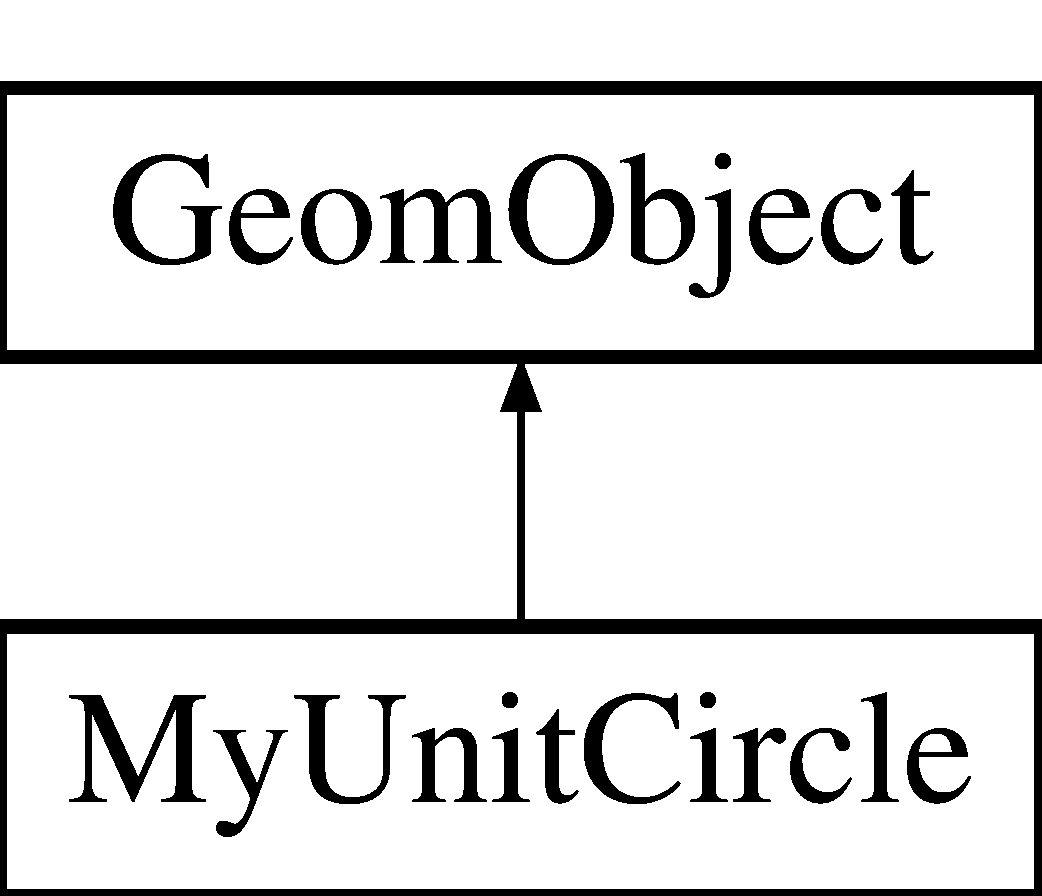
\includegraphics[height=2.000000cm]{classMyUnitCircle}
\end{center}
\end{figure}
\subsection*{Public Member Functions}
\begin{DoxyCompactItemize}
\item 
\hyperlink{classMyUnitCircle_a056add64776e52a8ea2ba2e9d6d0e32d}{My\+Unit\+Circle} ()
\begin{DoxyCompactList}\small\item\em Constructor\+: The circle is a 1D object (i.\+e. it\textquotesingle{}s parametrised by one intrinsic coordinate) in 2D space. Pass these arguments to the constructor of the Geom\+Object base class. \end{DoxyCompactList}\item 
virtual \hyperlink{classMyUnitCircle_ae6b321a25ef6f6b12d7c9a225f91140d}{$\sim$\+My\+Unit\+Circle} ()
\begin{DoxyCompactList}\small\item\em Destructor\+: Empty. \end{DoxyCompactList}\item 
void \hyperlink{classMyUnitCircle_ab60b73d1c28b013c40dd2aaa98072261}{position} (const Vector$<$ double $>$ \&xi, Vector$<$ double $>$ \&r) const
\begin{DoxyCompactList}\small\item\em Current position vector to material point at Lagrangian coordinate xi. \end{DoxyCompactList}\item 
void \hyperlink{classMyUnitCircle_a6a38e6320399940db4c9858668189ec3}{position} (const unsigned \&t, const Vector$<$ double $>$ \&xi, Vector$<$ double $>$ \&r) const
\begin{DoxyCompactList}\small\item\em Parametrised position on object\+: r(xi). Evaluated at previous time level. t=0\+: current time; t$>$0\+: previous time level. Circle is fixed -- simply call the steady version. \end{DoxyCompactList}\end{DoxyCompactItemize}


\subsection{Detailed Description}
Unit circle as Geom\+Object \[ x = \cos(\xi) \] \[ y = \sin(\xi) \]. 

Definition at line 57 of file two\+\_\+d\+\_\+unsteady\+\_\+heat\+\_\+adapt.\+cc.



\subsection{Constructor \& Destructor Documentation}
\mbox{\Hypertarget{classMyUnitCircle_a056add64776e52a8ea2ba2e9d6d0e32d}\label{classMyUnitCircle_a056add64776e52a8ea2ba2e9d6d0e32d}} 
\index{My\+Unit\+Circle@{My\+Unit\+Circle}!My\+Unit\+Circle@{My\+Unit\+Circle}}
\index{My\+Unit\+Circle@{My\+Unit\+Circle}!My\+Unit\+Circle@{My\+Unit\+Circle}}
\subsubsection{\texorpdfstring{My\+Unit\+Circle()}{MyUnitCircle()}}
{\footnotesize\ttfamily My\+Unit\+Circle\+::\+My\+Unit\+Circle (\begin{DoxyParamCaption}{ }\end{DoxyParamCaption})\hspace{0.3cm}{\ttfamily [inline]}}



Constructor\+: The circle is a 1D object (i.\+e. it\textquotesingle{}s parametrised by one intrinsic coordinate) in 2D space. Pass these arguments to the constructor of the Geom\+Object base class. 



Definition at line 65 of file two\+\_\+d\+\_\+unsteady\+\_\+heat\+\_\+adapt.\+cc.

\mbox{\Hypertarget{classMyUnitCircle_ae6b321a25ef6f6b12d7c9a225f91140d}\label{classMyUnitCircle_ae6b321a25ef6f6b12d7c9a225f91140d}} 
\index{My\+Unit\+Circle@{My\+Unit\+Circle}!````~My\+Unit\+Circle@{$\sim$\+My\+Unit\+Circle}}
\index{````~My\+Unit\+Circle@{$\sim$\+My\+Unit\+Circle}!My\+Unit\+Circle@{My\+Unit\+Circle}}
\subsubsection{\texorpdfstring{$\sim$\+My\+Unit\+Circle()}{~MyUnitCircle()}}
{\footnotesize\ttfamily virtual My\+Unit\+Circle\+::$\sim$\+My\+Unit\+Circle (\begin{DoxyParamCaption}{ }\end{DoxyParamCaption})\hspace{0.3cm}{\ttfamily [inline]}, {\ttfamily [virtual]}}



Destructor\+: Empty. 



Definition at line 68 of file two\+\_\+d\+\_\+unsteady\+\_\+heat\+\_\+adapt.\+cc.



\subsection{Member Function Documentation}
\mbox{\Hypertarget{classMyUnitCircle_ab60b73d1c28b013c40dd2aaa98072261}\label{classMyUnitCircle_ab60b73d1c28b013c40dd2aaa98072261}} 
\index{My\+Unit\+Circle@{My\+Unit\+Circle}!position@{position}}
\index{position@{position}!My\+Unit\+Circle@{My\+Unit\+Circle}}
\subsubsection{\texorpdfstring{position()}{position()}\hspace{0.1cm}{\footnotesize\ttfamily [1/2]}}
{\footnotesize\ttfamily void My\+Unit\+Circle\+::position (\begin{DoxyParamCaption}\item[{const Vector$<$ double $>$ \&}]{xi,  }\item[{Vector$<$ double $>$ \&}]{r }\end{DoxyParamCaption}) const\hspace{0.3cm}{\ttfamily [inline]}}



Current position vector to material point at Lagrangian coordinate xi. 



Definition at line 72 of file two\+\_\+d\+\_\+unsteady\+\_\+heat\+\_\+adapt.\+cc.

\mbox{\Hypertarget{classMyUnitCircle_a6a38e6320399940db4c9858668189ec3}\label{classMyUnitCircle_a6a38e6320399940db4c9858668189ec3}} 
\index{My\+Unit\+Circle@{My\+Unit\+Circle}!position@{position}}
\index{position@{position}!My\+Unit\+Circle@{My\+Unit\+Circle}}
\subsubsection{\texorpdfstring{position()}{position()}\hspace{0.1cm}{\footnotesize\ttfamily [2/2]}}
{\footnotesize\ttfamily void My\+Unit\+Circle\+::position (\begin{DoxyParamCaption}\item[{const unsigned \&}]{t,  }\item[{const Vector$<$ double $>$ \&}]{xi,  }\item[{Vector$<$ double $>$ \&}]{r }\end{DoxyParamCaption}) const\hspace{0.3cm}{\ttfamily [inline]}}



Parametrised position on object\+: r(xi). Evaluated at previous time level. t=0\+: current time; t$>$0\+: previous time level. Circle is fixed -- simply call the steady version. 



Definition at line 83 of file two\+\_\+d\+\_\+unsteady\+\_\+heat\+\_\+adapt.\+cc.



The documentation for this class was generated from the following file\+:\begin{DoxyCompactItemize}
\item 
\hyperlink{two__d__unsteady__heat__adapt_8cc}{two\+\_\+d\+\_\+unsteady\+\_\+heat\+\_\+adapt.\+cc}\end{DoxyCompactItemize}

\hypertarget{classRefineableUnsteadyHeatProblem}{}\section{Refineable\+Unsteady\+Heat\+Problem$<$ E\+L\+E\+M\+E\+NT $>$ Class Template Reference}
\label{classRefineableUnsteadyHeatProblem}\index{Refineable\+Unsteady\+Heat\+Problem$<$ E\+L\+E\+M\+E\+N\+T $>$@{Refineable\+Unsteady\+Heat\+Problem$<$ E\+L\+E\+M\+E\+N\+T $>$}}


Unsteady heat problem in quarter circle domain.  


Inheritance diagram for Refineable\+Unsteady\+Heat\+Problem$<$ E\+L\+E\+M\+E\+NT $>$\+:\begin{figure}[H]
\begin{center}
\leavevmode
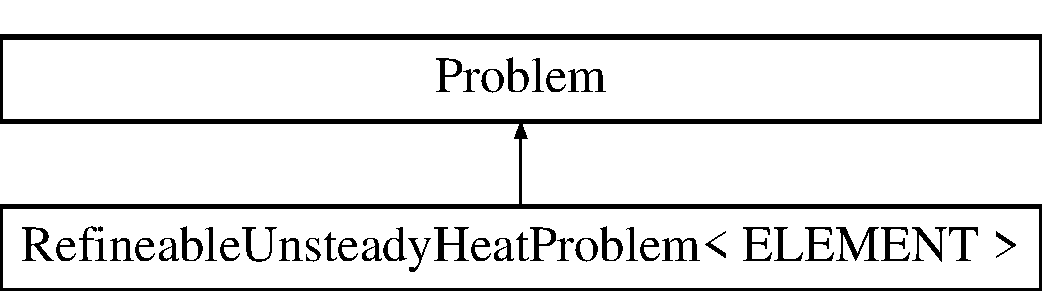
\includegraphics[height=2.000000cm]{classRefineableUnsteadyHeatProblem}
\end{center}
\end{figure}
\subsection*{Public Member Functions}
\begin{DoxyCompactItemize}
\item 
\hyperlink{classRefineableUnsteadyHeatProblem_a894f3bd6c1c23c307a736de6898e4e98}{Refineable\+Unsteady\+Heat\+Problem} (Unsteady\+Heat\+Equations$<$ 2 $>$\+::Unsteady\+Heat\+Source\+Fct\+Pt source\+\_\+fct\+\_\+pt)
\begin{DoxyCompactList}\small\item\em Constructor\+: Pass pointer to source function. \end{DoxyCompactList}\item 
\hyperlink{classRefineableUnsteadyHeatProblem_a975e00f5e87d77b4e1bf4d50482dea2b}{$\sim$\+Refineable\+Unsteady\+Heat\+Problem} ()
\begin{DoxyCompactList}\small\item\em Destructor\+: Close trace file. \end{DoxyCompactList}\item 
void \hyperlink{classRefineableUnsteadyHeatProblem_ada522772b79e92a75edf3724d0a273da}{actions\+\_\+after\+\_\+newton\+\_\+solve} ()
\begin{DoxyCompactList}\small\item\em Update the problem specs after solve (empty) \end{DoxyCompactList}\item 
void \hyperlink{classRefineableUnsteadyHeatProblem_aac1935e15c67b196e6db97dd058511b5}{actions\+\_\+before\+\_\+newton\+\_\+solve} ()
\begin{DoxyCompactList}\small\item\em Update the problem specs before solve (empty) \end{DoxyCompactList}\item 
void \hyperlink{classRefineableUnsteadyHeatProblem_aa740f2eb1b3909100a04709b401c0b41}{actions\+\_\+after\+\_\+implicit\+\_\+timestep} ()
\begin{DoxyCompactList}\small\item\em Update the problem specs after timestep (empty) \end{DoxyCompactList}\item 
void \hyperlink{classRefineableUnsteadyHeatProblem_ac754f1313cd6d684c149443beb5bcf9e}{actions\+\_\+before\+\_\+implicit\+\_\+timestep} ()
\begin{DoxyCompactList}\small\item\em Update the problem specs before next timestep\+: Set Dirchlet boundary conditions from exact solution. \end{DoxyCompactList}\item 
void \hyperlink{classRefineableUnsteadyHeatProblem_a4419fcea0ccbf0509f1d5dd37d8301de}{actions\+\_\+before\+\_\+adapt} ()
\begin{DoxyCompactList}\small\item\em Actions before adapt\+: Wipe the mesh of prescribed flux elements. \end{DoxyCompactList}\item 
void \hyperlink{classRefineableUnsteadyHeatProblem_a1f8a9e91269440c799a2075f989d62b1}{actions\+\_\+after\+\_\+adapt} ()
\begin{DoxyCompactList}\small\item\em Actions after adapt\+: Rebuild the mesh of prescribed flux elements. \end{DoxyCompactList}\item 
void \hyperlink{classRefineableUnsteadyHeatProblem_a30e2e1d62b059982f7014b74f4fe2be9}{set\+\_\+initial\+\_\+condition} ()
\begin{DoxyCompactList}\small\item\em Set initial condition (incl previous timesteps) according to specified function. Note that his overloads the virtual function in the Problem base class and is therefore executed automatically to re-\/assign the initial conditions during the spatially adaptive solution at the first timestep. \end{DoxyCompactList}\item 
void \hyperlink{classRefineableUnsteadyHeatProblem_a65601ec64c73ac578b43f4af04c46569}{create\+\_\+flux\+\_\+elements} (const unsigned \&b, Mesh $\ast$const \&\hyperlink{classRefineableUnsteadyHeatProblem_a4d8eec1505a3c53960a3182ec462b4e7}{bulk\+\_\+mesh\+\_\+pt}, Mesh $\ast$const \&surface\+\_\+mesh\+\_\+pt)
\begin{DoxyCompactList}\small\item\em Create Unsteady\+Heat flux elements on boundary b of the Mesh pointed to by bulk\+\_\+mesh\+\_\+pt and add them to the Mesh object pointed to by surface\+\_\+mesh\+\_\+pt. \end{DoxyCompactList}\item 
void \hyperlink{classRefineableUnsteadyHeatProblem_ad2e53af5c385e44e33e400b430b610e8}{delete\+\_\+flux\+\_\+elements} (Mesh $\ast$const \&surface\+\_\+mesh\+\_\+pt)
\begin{DoxyCompactList}\small\item\em Delete Unsteady\+Heat flux elements and wipe the surface mesh. \end{DoxyCompactList}\item 
void \hyperlink{classRefineableUnsteadyHeatProblem_a77d590171785b6b5f4070af9401c0e37}{doc\+\_\+solution} ()
\begin{DoxyCompactList}\small\item\em Doc the solution. \end{DoxyCompactList}\item 
void \hyperlink{classRefineableUnsteadyHeatProblem_a1fb939c3f9c258fd49328bb1516ced98}{dump\+\_\+it} (ofstream \&dump\+\_\+file)
\begin{DoxyCompactList}\small\item\em Dump problem data to allow for later restart. \end{DoxyCompactList}\item 
void \hyperlink{classRefineableUnsteadyHeatProblem_af36fa71e72852367411e21b50b179625}{restart} (ifstream \&restart\+\_\+file)
\begin{DoxyCompactList}\small\item\em Read problem data for restart. \end{DoxyCompactList}\item 
Refineable\+Quarter\+Circle\+Sector\+Mesh$<$ E\+L\+E\+M\+E\+NT $>$ $\ast$ \hyperlink{classRefineableUnsteadyHeatProblem_a4d8eec1505a3c53960a3182ec462b4e7}{bulk\+\_\+mesh\+\_\+pt} ()
\begin{DoxyCompactList}\small\item\em Pointer to bulk mesh. \end{DoxyCompactList}\end{DoxyCompactItemize}
\subsection*{Private Attributes}
\begin{DoxyCompactItemize}
\item 
Geom\+Object $\ast$ \hyperlink{classRefineableUnsteadyHeatProblem_a368512778fbfd59e918104340466b1df}{Boundary\+\_\+pt}
\begin{DoxyCompactList}\small\item\em Pointer to Geom\+Object that specifies the domain bondary. \end{DoxyCompactList}\item 
Unsteady\+Heat\+Equations$<$ 2 $>$\+::Unsteady\+Heat\+Source\+Fct\+Pt \hyperlink{classRefineableUnsteadyHeatProblem_a99eb5a2cd4b680b4f83e739bd4e16639}{Source\+\_\+fct\+\_\+pt}
\begin{DoxyCompactList}\small\item\em Pointer to source function. \end{DoxyCompactList}\item 
Refineable\+Quarter\+Circle\+Sector\+Mesh$<$ E\+L\+E\+M\+E\+NT $>$ $\ast$ \hyperlink{classRefineableUnsteadyHeatProblem_afade341e03a4c97e62444c80adc9552f}{Bulk\+\_\+mesh\+\_\+pt}
\begin{DoxyCompactList}\small\item\em Pointer to the \char`\"{}bulk\char`\"{} mesh. \end{DoxyCompactList}\item 
Mesh $\ast$ \hyperlink{classRefineableUnsteadyHeatProblem_a2febbb317a74e427bf6304235d779fe6}{Surface\+\_\+mesh\+\_\+pt}
\begin{DoxyCompactList}\small\item\em Pointer to the \char`\"{}surface\char`\"{} mesh. \end{DoxyCompactList}\item 
Node $\ast$ \hyperlink{classRefineableUnsteadyHeatProblem_a7ff1982af5819bab492c693178be0c24}{Doc\+\_\+node\+\_\+pt}
\begin{DoxyCompactList}\small\item\em Pointer to central node (exists at all refinement levels) for doc. \end{DoxyCompactList}\item 
Doc\+Info \hyperlink{classRefineableUnsteadyHeatProblem_a9ea9d79a57cb16a6292a637965767f7e}{Doc\+\_\+info}
\begin{DoxyCompactList}\small\item\em Doc info object. \end{DoxyCompactList}\item 
ofstream \hyperlink{classRefineableUnsteadyHeatProblem_a8f62ba78fb856d2e07b00254ca7a0e6a}{Trace\+\_\+file}
\begin{DoxyCompactList}\small\item\em Trace file. \end{DoxyCompactList}\end{DoxyCompactItemize}


\subsection{Detailed Description}
\subsubsection*{template$<$class E\+L\+E\+M\+E\+NT$>$\newline
class Refineable\+Unsteady\+Heat\+Problem$<$ E\+L\+E\+M\+E\+N\+T $>$}

Unsteady heat problem in quarter circle domain. 

Definition at line 191 of file two\+\_\+d\+\_\+unsteady\+\_\+heat\+\_\+adapt.\+cc.



\subsection{Constructor \& Destructor Documentation}
\mbox{\Hypertarget{classRefineableUnsteadyHeatProblem_a894f3bd6c1c23c307a736de6898e4e98}\label{classRefineableUnsteadyHeatProblem_a894f3bd6c1c23c307a736de6898e4e98}} 
\index{Refineable\+Unsteady\+Heat\+Problem@{Refineable\+Unsteady\+Heat\+Problem}!Refineable\+Unsteady\+Heat\+Problem@{Refineable\+Unsteady\+Heat\+Problem}}
\index{Refineable\+Unsteady\+Heat\+Problem@{Refineable\+Unsteady\+Heat\+Problem}!Refineable\+Unsteady\+Heat\+Problem@{Refineable\+Unsteady\+Heat\+Problem}}
\subsubsection{\texorpdfstring{Refineable\+Unsteady\+Heat\+Problem()}{RefineableUnsteadyHeatProblem()}}
{\footnotesize\ttfamily template$<$class E\+L\+E\+M\+E\+NT $>$ \\
\hyperlink{classRefineableUnsteadyHeatProblem}{Refineable\+Unsteady\+Heat\+Problem}$<$ E\+L\+E\+M\+E\+NT $>$\+::\hyperlink{classRefineableUnsteadyHeatProblem}{Refineable\+Unsteady\+Heat\+Problem} (\begin{DoxyParamCaption}\item[{Unsteady\+Heat\+Equations$<$ 2 $>$\+::Unsteady\+Heat\+Source\+Fct\+Pt}]{source\+\_\+fct\+\_\+pt }\end{DoxyParamCaption})}



Constructor\+: Pass pointer to source function. 

Constructor for Unsteady\+Heat problem in quarter circle domain. Pass pointer to source function. 

Definition at line 284 of file two\+\_\+d\+\_\+unsteady\+\_\+heat\+\_\+adapt.\+cc.



References Tanh\+Soln\+For\+Unsteady\+Heat\+::\+Alpha, Tanh\+Soln\+For\+Unsteady\+Heat\+::\+Beta, Refineable\+Unsteady\+Heat\+Problem$<$ E\+L\+E\+M\+E\+N\+T $>$\+::\+Boundary\+\_\+pt, Refineable\+Unsteady\+Heat\+Problem$<$ E\+L\+E\+M\+E\+N\+T $>$\+::\+Bulk\+\_\+mesh\+\_\+pt, Refineable\+Unsteady\+Heat\+Problem$<$ E\+L\+E\+M\+E\+N\+T $>$\+::create\+\_\+flux\+\_\+elements(), Refineable\+Unsteady\+Heat\+Problem$<$ E\+L\+E\+M\+E\+N\+T $>$\+::\+Doc\+\_\+info, Refineable\+Unsteady\+Heat\+Problem$<$ E\+L\+E\+M\+E\+N\+T $>$\+::\+Doc\+\_\+node\+\_\+pt, Tanh\+Soln\+For\+Unsteady\+Heat\+::\+Gamma, Tanh\+Soln\+For\+Unsteady\+Heat\+::prescribed\+\_\+flux\+\_\+on\+\_\+fixed\+\_\+y\+\_\+boundary(), Refineable\+Unsteady\+Heat\+Problem$<$ E\+L\+E\+M\+E\+N\+T $>$\+::\+Source\+\_\+fct\+\_\+pt, Refineable\+Unsteady\+Heat\+Problem$<$ E\+L\+E\+M\+E\+N\+T $>$\+::\+Surface\+\_\+mesh\+\_\+pt, Tanh\+Soln\+For\+Unsteady\+Heat\+::\+Tan\+Phi, and Refineable\+Unsteady\+Heat\+Problem$<$ E\+L\+E\+M\+E\+N\+T $>$\+::\+Trace\+\_\+file.

\mbox{\Hypertarget{classRefineableUnsteadyHeatProblem_a975e00f5e87d77b4e1bf4d50482dea2b}\label{classRefineableUnsteadyHeatProblem_a975e00f5e87d77b4e1bf4d50482dea2b}} 
\index{Refineable\+Unsteady\+Heat\+Problem@{Refineable\+Unsteady\+Heat\+Problem}!````~Refineable\+Unsteady\+Heat\+Problem@{$\sim$\+Refineable\+Unsteady\+Heat\+Problem}}
\index{````~Refineable\+Unsteady\+Heat\+Problem@{$\sim$\+Refineable\+Unsteady\+Heat\+Problem}!Refineable\+Unsteady\+Heat\+Problem@{Refineable\+Unsteady\+Heat\+Problem}}
\subsubsection{\texorpdfstring{$\sim$\+Refineable\+Unsteady\+Heat\+Problem()}{~RefineableUnsteadyHeatProblem()}}
{\footnotesize\ttfamily template$<$class E\+L\+E\+M\+E\+NT $>$ \\
\hyperlink{classRefineableUnsteadyHeatProblem}{Refineable\+Unsteady\+Heat\+Problem}$<$ E\+L\+E\+M\+E\+NT $>$\+::$\sim$\hyperlink{classRefineableUnsteadyHeatProblem}{Refineable\+Unsteady\+Heat\+Problem} (\begin{DoxyParamCaption}{ }\end{DoxyParamCaption})}



Destructor\+: Close trace file. 



Definition at line 439 of file two\+\_\+d\+\_\+unsteady\+\_\+heat\+\_\+adapt.\+cc.



References Refineable\+Unsteady\+Heat\+Problem$<$ E\+L\+E\+M\+E\+N\+T $>$\+::\+Trace\+\_\+file.



\subsection{Member Function Documentation}
\mbox{\Hypertarget{classRefineableUnsteadyHeatProblem_a1f8a9e91269440c799a2075f989d62b1}\label{classRefineableUnsteadyHeatProblem_a1f8a9e91269440c799a2075f989d62b1}} 
\index{Refineable\+Unsteady\+Heat\+Problem@{Refineable\+Unsteady\+Heat\+Problem}!actions\+\_\+after\+\_\+adapt@{actions\+\_\+after\+\_\+adapt}}
\index{actions\+\_\+after\+\_\+adapt@{actions\+\_\+after\+\_\+adapt}!Refineable\+Unsteady\+Heat\+Problem@{Refineable\+Unsteady\+Heat\+Problem}}
\subsubsection{\texorpdfstring{actions\+\_\+after\+\_\+adapt()}{actions\_after\_adapt()}}
{\footnotesize\ttfamily template$<$class E\+L\+E\+M\+E\+NT $>$ \\
void \hyperlink{classRefineableUnsteadyHeatProblem}{Refineable\+Unsteady\+Heat\+Problem}$<$ E\+L\+E\+M\+E\+NT $>$\+::actions\+\_\+after\+\_\+adapt (\begin{DoxyParamCaption}{ }\end{DoxyParamCaption})}



Actions after adapt\+: Rebuild the mesh of prescribed flux elements. 



Definition at line 500 of file two\+\_\+d\+\_\+unsteady\+\_\+heat\+\_\+adapt.\+cc.



References Refineable\+Unsteady\+Heat\+Problem$<$ E\+L\+E\+M\+E\+N\+T $>$\+::\+Bulk\+\_\+mesh\+\_\+pt, Refineable\+Unsteady\+Heat\+Problem$<$ E\+L\+E\+M\+E\+N\+T $>$\+::create\+\_\+flux\+\_\+elements(), Tanh\+Soln\+For\+Unsteady\+Heat\+::prescribed\+\_\+flux\+\_\+on\+\_\+fixed\+\_\+y\+\_\+boundary(), and Refineable\+Unsteady\+Heat\+Problem$<$ E\+L\+E\+M\+E\+N\+T $>$\+::\+Surface\+\_\+mesh\+\_\+pt.

\mbox{\Hypertarget{classRefineableUnsteadyHeatProblem_aa740f2eb1b3909100a04709b401c0b41}\label{classRefineableUnsteadyHeatProblem_aa740f2eb1b3909100a04709b401c0b41}} 
\index{Refineable\+Unsteady\+Heat\+Problem@{Refineable\+Unsteady\+Heat\+Problem}!actions\+\_\+after\+\_\+implicit\+\_\+timestep@{actions\+\_\+after\+\_\+implicit\+\_\+timestep}}
\index{actions\+\_\+after\+\_\+implicit\+\_\+timestep@{actions\+\_\+after\+\_\+implicit\+\_\+timestep}!Refineable\+Unsteady\+Heat\+Problem@{Refineable\+Unsteady\+Heat\+Problem}}
\subsubsection{\texorpdfstring{actions\+\_\+after\+\_\+implicit\+\_\+timestep()}{actions\_after\_implicit\_timestep()}}
{\footnotesize\ttfamily template$<$class E\+L\+E\+M\+E\+NT$>$ \\
void \hyperlink{classRefineableUnsteadyHeatProblem}{Refineable\+Unsteady\+Heat\+Problem}$<$ E\+L\+E\+M\+E\+NT $>$\+::actions\+\_\+after\+\_\+implicit\+\_\+timestep (\begin{DoxyParamCaption}{ }\end{DoxyParamCaption})\hspace{0.3cm}{\ttfamily [inline]}}



Update the problem specs after timestep (empty) 



Definition at line 210 of file two\+\_\+d\+\_\+unsteady\+\_\+heat\+\_\+adapt.\+cc.

\mbox{\Hypertarget{classRefineableUnsteadyHeatProblem_ada522772b79e92a75edf3724d0a273da}\label{classRefineableUnsteadyHeatProblem_ada522772b79e92a75edf3724d0a273da}} 
\index{Refineable\+Unsteady\+Heat\+Problem@{Refineable\+Unsteady\+Heat\+Problem}!actions\+\_\+after\+\_\+newton\+\_\+solve@{actions\+\_\+after\+\_\+newton\+\_\+solve}}
\index{actions\+\_\+after\+\_\+newton\+\_\+solve@{actions\+\_\+after\+\_\+newton\+\_\+solve}!Refineable\+Unsteady\+Heat\+Problem@{Refineable\+Unsteady\+Heat\+Problem}}
\subsubsection{\texorpdfstring{actions\+\_\+after\+\_\+newton\+\_\+solve()}{actions\_after\_newton\_solve()}}
{\footnotesize\ttfamily template$<$class E\+L\+E\+M\+E\+NT$>$ \\
void \hyperlink{classRefineableUnsteadyHeatProblem}{Refineable\+Unsteady\+Heat\+Problem}$<$ E\+L\+E\+M\+E\+NT $>$\+::actions\+\_\+after\+\_\+newton\+\_\+solve (\begin{DoxyParamCaption}{ }\end{DoxyParamCaption})\hspace{0.3cm}{\ttfamily [inline]}}



Update the problem specs after solve (empty) 



Definition at line 204 of file two\+\_\+d\+\_\+unsteady\+\_\+heat\+\_\+adapt.\+cc.

\mbox{\Hypertarget{classRefineableUnsteadyHeatProblem_a4419fcea0ccbf0509f1d5dd37d8301de}\label{classRefineableUnsteadyHeatProblem_a4419fcea0ccbf0509f1d5dd37d8301de}} 
\index{Refineable\+Unsteady\+Heat\+Problem@{Refineable\+Unsteady\+Heat\+Problem}!actions\+\_\+before\+\_\+adapt@{actions\+\_\+before\+\_\+adapt}}
\index{actions\+\_\+before\+\_\+adapt@{actions\+\_\+before\+\_\+adapt}!Refineable\+Unsteady\+Heat\+Problem@{Refineable\+Unsteady\+Heat\+Problem}}
\subsubsection{\texorpdfstring{actions\+\_\+before\+\_\+adapt()}{actions\_before\_adapt()}}
{\footnotesize\ttfamily template$<$class E\+L\+E\+M\+E\+NT $>$ \\
void \hyperlink{classRefineableUnsteadyHeatProblem}{Refineable\+Unsteady\+Heat\+Problem}$<$ E\+L\+E\+M\+E\+NT $>$\+::actions\+\_\+before\+\_\+adapt (\begin{DoxyParamCaption}{ }\end{DoxyParamCaption})}



Actions before adapt\+: Wipe the mesh of prescribed flux elements. 



Definition at line 484 of file two\+\_\+d\+\_\+unsteady\+\_\+heat\+\_\+adapt.\+cc.



References Refineable\+Unsteady\+Heat\+Problem$<$ E\+L\+E\+M\+E\+N\+T $>$\+::delete\+\_\+flux\+\_\+elements(), and Refineable\+Unsteady\+Heat\+Problem$<$ E\+L\+E\+M\+E\+N\+T $>$\+::\+Surface\+\_\+mesh\+\_\+pt.

\mbox{\Hypertarget{classRefineableUnsteadyHeatProblem_ac754f1313cd6d684c149443beb5bcf9e}\label{classRefineableUnsteadyHeatProblem_ac754f1313cd6d684c149443beb5bcf9e}} 
\index{Refineable\+Unsteady\+Heat\+Problem@{Refineable\+Unsteady\+Heat\+Problem}!actions\+\_\+before\+\_\+implicit\+\_\+timestep@{actions\+\_\+before\+\_\+implicit\+\_\+timestep}}
\index{actions\+\_\+before\+\_\+implicit\+\_\+timestep@{actions\+\_\+before\+\_\+implicit\+\_\+timestep}!Refineable\+Unsteady\+Heat\+Problem@{Refineable\+Unsteady\+Heat\+Problem}}
\subsubsection{\texorpdfstring{actions\+\_\+before\+\_\+implicit\+\_\+timestep()}{actions\_before\_implicit\_timestep()}}
{\footnotesize\ttfamily template$<$class E\+L\+E\+M\+E\+NT $>$ \\
void \hyperlink{classRefineableUnsteadyHeatProblem}{Refineable\+Unsteady\+Heat\+Problem}$<$ E\+L\+E\+M\+E\+NT $>$\+::actions\+\_\+before\+\_\+implicit\+\_\+timestep (\begin{DoxyParamCaption}{ }\end{DoxyParamCaption})}



Update the problem specs before next timestep\+: Set Dirchlet boundary conditions from exact solution. 

Actions before timestep\+: Set the boundary conditions for the current time. 

Definition at line 451 of file two\+\_\+d\+\_\+unsteady\+\_\+heat\+\_\+adapt.\+cc.



References Refineable\+Unsteady\+Heat\+Problem$<$ E\+L\+E\+M\+E\+N\+T $>$\+::\+Bulk\+\_\+mesh\+\_\+pt, and Tanh\+Soln\+For\+Unsteady\+Heat\+::get\+\_\+exact\+\_\+u().

\mbox{\Hypertarget{classRefineableUnsteadyHeatProblem_aac1935e15c67b196e6db97dd058511b5}\label{classRefineableUnsteadyHeatProblem_aac1935e15c67b196e6db97dd058511b5}} 
\index{Refineable\+Unsteady\+Heat\+Problem@{Refineable\+Unsteady\+Heat\+Problem}!actions\+\_\+before\+\_\+newton\+\_\+solve@{actions\+\_\+before\+\_\+newton\+\_\+solve}}
\index{actions\+\_\+before\+\_\+newton\+\_\+solve@{actions\+\_\+before\+\_\+newton\+\_\+solve}!Refineable\+Unsteady\+Heat\+Problem@{Refineable\+Unsteady\+Heat\+Problem}}
\subsubsection{\texorpdfstring{actions\+\_\+before\+\_\+newton\+\_\+solve()}{actions\_before\_newton\_solve()}}
{\footnotesize\ttfamily template$<$class E\+L\+E\+M\+E\+NT$>$ \\
void \hyperlink{classRefineableUnsteadyHeatProblem}{Refineable\+Unsteady\+Heat\+Problem}$<$ E\+L\+E\+M\+E\+NT $>$\+::actions\+\_\+before\+\_\+newton\+\_\+solve (\begin{DoxyParamCaption}{ }\end{DoxyParamCaption})\hspace{0.3cm}{\ttfamily [inline]}}



Update the problem specs before solve (empty) 



Definition at line 207 of file two\+\_\+d\+\_\+unsteady\+\_\+heat\+\_\+adapt.\+cc.

\mbox{\Hypertarget{classRefineableUnsteadyHeatProblem_a4d8eec1505a3c53960a3182ec462b4e7}\label{classRefineableUnsteadyHeatProblem_a4d8eec1505a3c53960a3182ec462b4e7}} 
\index{Refineable\+Unsteady\+Heat\+Problem@{Refineable\+Unsteady\+Heat\+Problem}!bulk\+\_\+mesh\+\_\+pt@{bulk\+\_\+mesh\+\_\+pt}}
\index{bulk\+\_\+mesh\+\_\+pt@{bulk\+\_\+mesh\+\_\+pt}!Refineable\+Unsteady\+Heat\+Problem@{Refineable\+Unsteady\+Heat\+Problem}}
\subsubsection{\texorpdfstring{bulk\+\_\+mesh\+\_\+pt()}{bulk\_mesh\_pt()}}
{\footnotesize\ttfamily template$<$class E\+L\+E\+M\+E\+NT$>$ \\
Refineable\+Quarter\+Circle\+Sector\+Mesh$<$E\+L\+E\+M\+E\+NT$>$$\ast$ \hyperlink{classRefineableUnsteadyHeatProblem}{Refineable\+Unsteady\+Heat\+Problem}$<$ E\+L\+E\+M\+E\+NT $>$\+::bulk\+\_\+mesh\+\_\+pt (\begin{DoxyParamCaption}{ }\end{DoxyParamCaption})\hspace{0.3cm}{\ttfamily [inline]}}



Pointer to bulk mesh. 



Definition at line 248 of file two\+\_\+d\+\_\+unsteady\+\_\+heat\+\_\+adapt.\+cc.



Referenced by main().

\mbox{\Hypertarget{classRefineableUnsteadyHeatProblem_a65601ec64c73ac578b43f4af04c46569}\label{classRefineableUnsteadyHeatProblem_a65601ec64c73ac578b43f4af04c46569}} 
\index{Refineable\+Unsteady\+Heat\+Problem@{Refineable\+Unsteady\+Heat\+Problem}!create\+\_\+flux\+\_\+elements@{create\+\_\+flux\+\_\+elements}}
\index{create\+\_\+flux\+\_\+elements@{create\+\_\+flux\+\_\+elements}!Refineable\+Unsteady\+Heat\+Problem@{Refineable\+Unsteady\+Heat\+Problem}}
\subsubsection{\texorpdfstring{create\+\_\+flux\+\_\+elements()}{create\_flux\_elements()}}
{\footnotesize\ttfamily template$<$class E\+L\+E\+M\+E\+NT $>$ \\
void \hyperlink{classRefineableUnsteadyHeatProblem}{Refineable\+Unsteady\+Heat\+Problem}$<$ E\+L\+E\+M\+E\+NT $>$\+::create\+\_\+flux\+\_\+elements (\begin{DoxyParamCaption}\item[{const unsigned \&}]{b,  }\item[{Mesh $\ast$const \&}]{bulk\+\_\+mesh\+\_\+pt,  }\item[{Mesh $\ast$const \&}]{surface\+\_\+mesh\+\_\+pt }\end{DoxyParamCaption})}



Create Unsteady\+Heat flux elements on boundary b of the Mesh pointed to by bulk\+\_\+mesh\+\_\+pt and add them to the Mesh object pointed to by surface\+\_\+mesh\+\_\+pt. 

Create Unsteady\+Heat Flux Elements on the b-\/th boundary of the Mesh object pointed to by bulk\+\_\+mesh\+\_\+pt and add the elements to the Mesh object pointed to by surface\+\_\+mesh\+\_\+pt. 

Definition at line 803 of file two\+\_\+d\+\_\+unsteady\+\_\+heat\+\_\+adapt.\+cc.



References Refineable\+Unsteady\+Heat\+Problem$<$ E\+L\+E\+M\+E\+N\+T $>$\+::delete\+\_\+flux\+\_\+elements().



Referenced by Refineable\+Unsteady\+Heat\+Problem$<$ E\+L\+E\+M\+E\+N\+T $>$\+::actions\+\_\+after\+\_\+adapt(), Refineable\+Unsteady\+Heat\+Problem$<$ E\+L\+E\+M\+E\+N\+T $>$\+::doc\+\_\+solution(), and Refineable\+Unsteady\+Heat\+Problem$<$ E\+L\+E\+M\+E\+N\+T $>$\+::\+Refineable\+Unsteady\+Heat\+Problem().

\mbox{\Hypertarget{classRefineableUnsteadyHeatProblem_ad2e53af5c385e44e33e400b430b610e8}\label{classRefineableUnsteadyHeatProblem_ad2e53af5c385e44e33e400b430b610e8}} 
\index{Refineable\+Unsteady\+Heat\+Problem@{Refineable\+Unsteady\+Heat\+Problem}!delete\+\_\+flux\+\_\+elements@{delete\+\_\+flux\+\_\+elements}}
\index{delete\+\_\+flux\+\_\+elements@{delete\+\_\+flux\+\_\+elements}!Refineable\+Unsteady\+Heat\+Problem@{Refineable\+Unsteady\+Heat\+Problem}}
\subsubsection{\texorpdfstring{delete\+\_\+flux\+\_\+elements()}{delete\_flux\_elements()}}
{\footnotesize\ttfamily template$<$class E\+L\+E\+M\+E\+NT $>$ \\
void \hyperlink{classRefineableUnsteadyHeatProblem}{Refineable\+Unsteady\+Heat\+Problem}$<$ E\+L\+E\+M\+E\+NT $>$\+::delete\+\_\+flux\+\_\+elements (\begin{DoxyParamCaption}\item[{Mesh $\ast$const \&}]{surface\+\_\+mesh\+\_\+pt }\end{DoxyParamCaption})}



Delete Unsteady\+Heat flux elements and wipe the surface mesh. 

Delete Unsteady\+Heat Flux Elements and wipe the surface mesh. 

Definition at line 836 of file two\+\_\+d\+\_\+unsteady\+\_\+heat\+\_\+adapt.\+cc.



Referenced by Refineable\+Unsteady\+Heat\+Problem$<$ E\+L\+E\+M\+E\+N\+T $>$\+::actions\+\_\+before\+\_\+adapt(), and Refineable\+Unsteady\+Heat\+Problem$<$ E\+L\+E\+M\+E\+N\+T $>$\+::create\+\_\+flux\+\_\+elements().

\mbox{\Hypertarget{classRefineableUnsteadyHeatProblem_a77d590171785b6b5f4070af9401c0e37}\label{classRefineableUnsteadyHeatProblem_a77d590171785b6b5f4070af9401c0e37}} 
\index{Refineable\+Unsteady\+Heat\+Problem@{Refineable\+Unsteady\+Heat\+Problem}!doc\+\_\+solution@{doc\+\_\+solution}}
\index{doc\+\_\+solution@{doc\+\_\+solution}!Refineable\+Unsteady\+Heat\+Problem@{Refineable\+Unsteady\+Heat\+Problem}}
\subsubsection{\texorpdfstring{doc\+\_\+solution()}{doc\_solution()}}
{\footnotesize\ttfamily template$<$class E\+L\+E\+M\+E\+NT $>$ \\
void \hyperlink{classRefineableUnsteadyHeatProblem}{Refineable\+Unsteady\+Heat\+Problem}$<$ E\+L\+E\+M\+E\+NT $>$\+::doc\+\_\+solution (\begin{DoxyParamCaption}{ }\end{DoxyParamCaption})}



Doc the solution. 



Definition at line 662 of file two\+\_\+d\+\_\+unsteady\+\_\+heat\+\_\+adapt.\+cc.



References Refineable\+Unsteady\+Heat\+Problem$<$ E\+L\+E\+M\+E\+N\+T $>$\+::\+Boundary\+\_\+pt, Refineable\+Unsteady\+Heat\+Problem$<$ E\+L\+E\+M\+E\+N\+T $>$\+::\+Bulk\+\_\+mesh\+\_\+pt, Refineable\+Unsteady\+Heat\+Problem$<$ E\+L\+E\+M\+E\+N\+T $>$\+::create\+\_\+flux\+\_\+elements(), Refineable\+Unsteady\+Heat\+Problem$<$ E\+L\+E\+M\+E\+N\+T $>$\+::\+Doc\+\_\+info, Refineable\+Unsteady\+Heat\+Problem$<$ E\+L\+E\+M\+E\+N\+T $>$\+::\+Doc\+\_\+node\+\_\+pt, Refineable\+Unsteady\+Heat\+Problem$<$ E\+L\+E\+M\+E\+N\+T $>$\+::dump\+\_\+it(), Tanh\+Soln\+For\+Unsteady\+Heat\+::get\+\_\+exact\+\_\+u(), Tanh\+Soln\+For\+Unsteady\+Heat\+::step\+\_\+position(), and Refineable\+Unsteady\+Heat\+Problem$<$ E\+L\+E\+M\+E\+N\+T $>$\+::\+Trace\+\_\+file.



Referenced by main().

\mbox{\Hypertarget{classRefineableUnsteadyHeatProblem_a1fb939c3f9c258fd49328bb1516ced98}\label{classRefineableUnsteadyHeatProblem_a1fb939c3f9c258fd49328bb1516ced98}} 
\index{Refineable\+Unsteady\+Heat\+Problem@{Refineable\+Unsteady\+Heat\+Problem}!dump\+\_\+it@{dump\+\_\+it}}
\index{dump\+\_\+it@{dump\+\_\+it}!Refineable\+Unsteady\+Heat\+Problem@{Refineable\+Unsteady\+Heat\+Problem}}
\subsubsection{\texorpdfstring{dump\+\_\+it()}{dump\_it()}}
{\footnotesize\ttfamily template$<$class E\+L\+E\+M\+E\+NT $>$ \\
void \hyperlink{classRefineableUnsteadyHeatProblem}{Refineable\+Unsteady\+Heat\+Problem}$<$ E\+L\+E\+M\+E\+NT $>$\+::dump\+\_\+it (\begin{DoxyParamCaption}\item[{ofstream \&}]{dump\+\_\+file }\end{DoxyParamCaption})}



Dump problem data to allow for later restart. 

Dump the solution to disk. 

Definition at line 858 of file two\+\_\+d\+\_\+unsteady\+\_\+heat\+\_\+adapt.\+cc.



Referenced by Refineable\+Unsteady\+Heat\+Problem$<$ E\+L\+E\+M\+E\+N\+T $>$\+::doc\+\_\+solution().

\mbox{\Hypertarget{classRefineableUnsteadyHeatProblem_af36fa71e72852367411e21b50b179625}\label{classRefineableUnsteadyHeatProblem_af36fa71e72852367411e21b50b179625}} 
\index{Refineable\+Unsteady\+Heat\+Problem@{Refineable\+Unsteady\+Heat\+Problem}!restart@{restart}}
\index{restart@{restart}!Refineable\+Unsteady\+Heat\+Problem@{Refineable\+Unsteady\+Heat\+Problem}}
\subsubsection{\texorpdfstring{restart()}{restart()}}
{\footnotesize\ttfamily template$<$class E\+L\+E\+M\+E\+NT $>$ \\
void \hyperlink{classRefineableUnsteadyHeatProblem}{Refineable\+Unsteady\+Heat\+Problem}$<$ E\+L\+E\+M\+E\+NT $>$\+::restart (\begin{DoxyParamCaption}\item[{ifstream \&}]{restart\+\_\+file }\end{DoxyParamCaption})}



Read problem data for restart. 

Read solution from disk. 

Definition at line 869 of file two\+\_\+d\+\_\+unsteady\+\_\+heat\+\_\+adapt.\+cc.



Referenced by Refineable\+Unsteady\+Heat\+Problem$<$ E\+L\+E\+M\+E\+N\+T $>$\+::set\+\_\+initial\+\_\+condition().

\mbox{\Hypertarget{classRefineableUnsteadyHeatProblem_a30e2e1d62b059982f7014b74f4fe2be9}\label{classRefineableUnsteadyHeatProblem_a30e2e1d62b059982f7014b74f4fe2be9}} 
\index{Refineable\+Unsteady\+Heat\+Problem@{Refineable\+Unsteady\+Heat\+Problem}!set\+\_\+initial\+\_\+condition@{set\+\_\+initial\+\_\+condition}}
\index{set\+\_\+initial\+\_\+condition@{set\+\_\+initial\+\_\+condition}!Refineable\+Unsteady\+Heat\+Problem@{Refineable\+Unsteady\+Heat\+Problem}}
\subsubsection{\texorpdfstring{set\+\_\+initial\+\_\+condition()}{set\_initial\_condition()}}
{\footnotesize\ttfamily template$<$class E\+L\+E\+M\+E\+NT $>$ \\
void \hyperlink{classRefineableUnsteadyHeatProblem}{Refineable\+Unsteady\+Heat\+Problem}$<$ E\+L\+E\+M\+E\+NT $>$\+::set\+\_\+initial\+\_\+condition (\begin{DoxyParamCaption}{ }\end{DoxyParamCaption})}



Set initial condition (incl previous timesteps) according to specified function. Note that his overloads the virtual function in the Problem base class and is therefore executed automatically to re-\/assign the initial conditions during the spatially adaptive solution at the first timestep. 

Set initial condition\+: Assign previous and current values from exact solution. 

Definition at line 530 of file two\+\_\+d\+\_\+unsteady\+\_\+heat\+\_\+adapt.\+cc.



References Refineable\+Unsteady\+Heat\+Problem$<$ E\+L\+E\+M\+E\+N\+T $>$\+::\+Bulk\+\_\+mesh\+\_\+pt, Tanh\+Soln\+For\+Unsteady\+Heat\+::get\+\_\+exact\+\_\+u(), and Refineable\+Unsteady\+Heat\+Problem$<$ E\+L\+E\+M\+E\+N\+T $>$\+::restart().



Referenced by main().



\subsection{Member Data Documentation}
\mbox{\Hypertarget{classRefineableUnsteadyHeatProblem_a368512778fbfd59e918104340466b1df}\label{classRefineableUnsteadyHeatProblem_a368512778fbfd59e918104340466b1df}} 
\index{Refineable\+Unsteady\+Heat\+Problem@{Refineable\+Unsteady\+Heat\+Problem}!Boundary\+\_\+pt@{Boundary\+\_\+pt}}
\index{Boundary\+\_\+pt@{Boundary\+\_\+pt}!Refineable\+Unsteady\+Heat\+Problem@{Refineable\+Unsteady\+Heat\+Problem}}
\subsubsection{\texorpdfstring{Boundary\+\_\+pt}{Boundary\_pt}}
{\footnotesize\ttfamily template$<$class E\+L\+E\+M\+E\+NT$>$ \\
Geom\+Object$\ast$ \hyperlink{classRefineableUnsteadyHeatProblem}{Refineable\+Unsteady\+Heat\+Problem}$<$ E\+L\+E\+M\+E\+NT $>$\+::Boundary\+\_\+pt\hspace{0.3cm}{\ttfamily [private]}}



Pointer to Geom\+Object that specifies the domain bondary. 



Definition at line 257 of file two\+\_\+d\+\_\+unsteady\+\_\+heat\+\_\+adapt.\+cc.



Referenced by Refineable\+Unsteady\+Heat\+Problem$<$ E\+L\+E\+M\+E\+N\+T $>$\+::doc\+\_\+solution(), and Refineable\+Unsteady\+Heat\+Problem$<$ E\+L\+E\+M\+E\+N\+T $>$\+::\+Refineable\+Unsteady\+Heat\+Problem().

\mbox{\Hypertarget{classRefineableUnsteadyHeatProblem_afade341e03a4c97e62444c80adc9552f}\label{classRefineableUnsteadyHeatProblem_afade341e03a4c97e62444c80adc9552f}} 
\index{Refineable\+Unsteady\+Heat\+Problem@{Refineable\+Unsteady\+Heat\+Problem}!Bulk\+\_\+mesh\+\_\+pt@{Bulk\+\_\+mesh\+\_\+pt}}
\index{Bulk\+\_\+mesh\+\_\+pt@{Bulk\+\_\+mesh\+\_\+pt}!Refineable\+Unsteady\+Heat\+Problem@{Refineable\+Unsteady\+Heat\+Problem}}
\subsubsection{\texorpdfstring{Bulk\+\_\+mesh\+\_\+pt}{Bulk\_mesh\_pt}}
{\footnotesize\ttfamily template$<$class E\+L\+E\+M\+E\+NT$>$ \\
Refineable\+Quarter\+Circle\+Sector\+Mesh$<$E\+L\+E\+M\+E\+NT$>$$\ast$ \hyperlink{classRefineableUnsteadyHeatProblem}{Refineable\+Unsteady\+Heat\+Problem}$<$ E\+L\+E\+M\+E\+NT $>$\+::Bulk\+\_\+mesh\+\_\+pt\hspace{0.3cm}{\ttfamily [private]}}



Pointer to the \char`\"{}bulk\char`\"{} mesh. 



Definition at line 263 of file two\+\_\+d\+\_\+unsteady\+\_\+heat\+\_\+adapt.\+cc.



Referenced by Refineable\+Unsteady\+Heat\+Problem$<$ E\+L\+E\+M\+E\+N\+T $>$\+::actions\+\_\+after\+\_\+adapt(), Refineable\+Unsteady\+Heat\+Problem$<$ E\+L\+E\+M\+E\+N\+T $>$\+::actions\+\_\+before\+\_\+implicit\+\_\+timestep(), Refineable\+Unsteady\+Heat\+Problem$<$ E\+L\+E\+M\+E\+N\+T $>$\+::doc\+\_\+solution(), Refineable\+Unsteady\+Heat\+Problem$<$ E\+L\+E\+M\+E\+N\+T $>$\+::\+Refineable\+Unsteady\+Heat\+Problem(), and Refineable\+Unsteady\+Heat\+Problem$<$ E\+L\+E\+M\+E\+N\+T $>$\+::set\+\_\+initial\+\_\+condition().

\mbox{\Hypertarget{classRefineableUnsteadyHeatProblem_a9ea9d79a57cb16a6292a637965767f7e}\label{classRefineableUnsteadyHeatProblem_a9ea9d79a57cb16a6292a637965767f7e}} 
\index{Refineable\+Unsteady\+Heat\+Problem@{Refineable\+Unsteady\+Heat\+Problem}!Doc\+\_\+info@{Doc\+\_\+info}}
\index{Doc\+\_\+info@{Doc\+\_\+info}!Refineable\+Unsteady\+Heat\+Problem@{Refineable\+Unsteady\+Heat\+Problem}}
\subsubsection{\texorpdfstring{Doc\+\_\+info}{Doc\_info}}
{\footnotesize\ttfamily template$<$class E\+L\+E\+M\+E\+NT$>$ \\
Doc\+Info \hyperlink{classRefineableUnsteadyHeatProblem}{Refineable\+Unsteady\+Heat\+Problem}$<$ E\+L\+E\+M\+E\+NT $>$\+::Doc\+\_\+info\hspace{0.3cm}{\ttfamily [private]}}



Doc info object. 



Definition at line 272 of file two\+\_\+d\+\_\+unsteady\+\_\+heat\+\_\+adapt.\+cc.



Referenced by Refineable\+Unsteady\+Heat\+Problem$<$ E\+L\+E\+M\+E\+N\+T $>$\+::doc\+\_\+solution(), and Refineable\+Unsteady\+Heat\+Problem$<$ E\+L\+E\+M\+E\+N\+T $>$\+::\+Refineable\+Unsteady\+Heat\+Problem().

\mbox{\Hypertarget{classRefineableUnsteadyHeatProblem_a7ff1982af5819bab492c693178be0c24}\label{classRefineableUnsteadyHeatProblem_a7ff1982af5819bab492c693178be0c24}} 
\index{Refineable\+Unsteady\+Heat\+Problem@{Refineable\+Unsteady\+Heat\+Problem}!Doc\+\_\+node\+\_\+pt@{Doc\+\_\+node\+\_\+pt}}
\index{Doc\+\_\+node\+\_\+pt@{Doc\+\_\+node\+\_\+pt}!Refineable\+Unsteady\+Heat\+Problem@{Refineable\+Unsteady\+Heat\+Problem}}
\subsubsection{\texorpdfstring{Doc\+\_\+node\+\_\+pt}{Doc\_node\_pt}}
{\footnotesize\ttfamily template$<$class E\+L\+E\+M\+E\+NT$>$ \\
Node$\ast$ \hyperlink{classRefineableUnsteadyHeatProblem}{Refineable\+Unsteady\+Heat\+Problem}$<$ E\+L\+E\+M\+E\+NT $>$\+::Doc\+\_\+node\+\_\+pt\hspace{0.3cm}{\ttfamily [private]}}



Pointer to central node (exists at all refinement levels) for doc. 



Definition at line 269 of file two\+\_\+d\+\_\+unsteady\+\_\+heat\+\_\+adapt.\+cc.



Referenced by Refineable\+Unsteady\+Heat\+Problem$<$ E\+L\+E\+M\+E\+N\+T $>$\+::doc\+\_\+solution(), and Refineable\+Unsteady\+Heat\+Problem$<$ E\+L\+E\+M\+E\+N\+T $>$\+::\+Refineable\+Unsteady\+Heat\+Problem().

\mbox{\Hypertarget{classRefineableUnsteadyHeatProblem_a99eb5a2cd4b680b4f83e739bd4e16639}\label{classRefineableUnsteadyHeatProblem_a99eb5a2cd4b680b4f83e739bd4e16639}} 
\index{Refineable\+Unsteady\+Heat\+Problem@{Refineable\+Unsteady\+Heat\+Problem}!Source\+\_\+fct\+\_\+pt@{Source\+\_\+fct\+\_\+pt}}
\index{Source\+\_\+fct\+\_\+pt@{Source\+\_\+fct\+\_\+pt}!Refineable\+Unsteady\+Heat\+Problem@{Refineable\+Unsteady\+Heat\+Problem}}
\subsubsection{\texorpdfstring{Source\+\_\+fct\+\_\+pt}{Source\_fct\_pt}}
{\footnotesize\ttfamily template$<$class E\+L\+E\+M\+E\+NT$>$ \\
Unsteady\+Heat\+Equations$<$2$>$\+::Unsteady\+Heat\+Source\+Fct\+Pt \hyperlink{classRefineableUnsteadyHeatProblem}{Refineable\+Unsteady\+Heat\+Problem}$<$ E\+L\+E\+M\+E\+NT $>$\+::Source\+\_\+fct\+\_\+pt\hspace{0.3cm}{\ttfamily [private]}}



Pointer to source function. 



Definition at line 260 of file two\+\_\+d\+\_\+unsteady\+\_\+heat\+\_\+adapt.\+cc.



Referenced by Refineable\+Unsteady\+Heat\+Problem$<$ E\+L\+E\+M\+E\+N\+T $>$\+::\+Refineable\+Unsteady\+Heat\+Problem().

\mbox{\Hypertarget{classRefineableUnsteadyHeatProblem_a2febbb317a74e427bf6304235d779fe6}\label{classRefineableUnsteadyHeatProblem_a2febbb317a74e427bf6304235d779fe6}} 
\index{Refineable\+Unsteady\+Heat\+Problem@{Refineable\+Unsteady\+Heat\+Problem}!Surface\+\_\+mesh\+\_\+pt@{Surface\+\_\+mesh\+\_\+pt}}
\index{Surface\+\_\+mesh\+\_\+pt@{Surface\+\_\+mesh\+\_\+pt}!Refineable\+Unsteady\+Heat\+Problem@{Refineable\+Unsteady\+Heat\+Problem}}
\subsubsection{\texorpdfstring{Surface\+\_\+mesh\+\_\+pt}{Surface\_mesh\_pt}}
{\footnotesize\ttfamily template$<$class E\+L\+E\+M\+E\+NT$>$ \\
Mesh$\ast$ \hyperlink{classRefineableUnsteadyHeatProblem}{Refineable\+Unsteady\+Heat\+Problem}$<$ E\+L\+E\+M\+E\+NT $>$\+::Surface\+\_\+mesh\+\_\+pt\hspace{0.3cm}{\ttfamily [private]}}



Pointer to the \char`\"{}surface\char`\"{} mesh. 



Definition at line 266 of file two\+\_\+d\+\_\+unsteady\+\_\+heat\+\_\+adapt.\+cc.



Referenced by Refineable\+Unsteady\+Heat\+Problem$<$ E\+L\+E\+M\+E\+N\+T $>$\+::actions\+\_\+after\+\_\+adapt(), Refineable\+Unsteady\+Heat\+Problem$<$ E\+L\+E\+M\+E\+N\+T $>$\+::actions\+\_\+before\+\_\+adapt(), and Refineable\+Unsteady\+Heat\+Problem$<$ E\+L\+E\+M\+E\+N\+T $>$\+::\+Refineable\+Unsteady\+Heat\+Problem().

\mbox{\Hypertarget{classRefineableUnsteadyHeatProblem_a8f62ba78fb856d2e07b00254ca7a0e6a}\label{classRefineableUnsteadyHeatProblem_a8f62ba78fb856d2e07b00254ca7a0e6a}} 
\index{Refineable\+Unsteady\+Heat\+Problem@{Refineable\+Unsteady\+Heat\+Problem}!Trace\+\_\+file@{Trace\+\_\+file}}
\index{Trace\+\_\+file@{Trace\+\_\+file}!Refineable\+Unsteady\+Heat\+Problem@{Refineable\+Unsteady\+Heat\+Problem}}
\subsubsection{\texorpdfstring{Trace\+\_\+file}{Trace\_file}}
{\footnotesize\ttfamily template$<$class E\+L\+E\+M\+E\+NT$>$ \\
ofstream \hyperlink{classRefineableUnsteadyHeatProblem}{Refineable\+Unsteady\+Heat\+Problem}$<$ E\+L\+E\+M\+E\+NT $>$\+::Trace\+\_\+file\hspace{0.3cm}{\ttfamily [private]}}



Trace file. 



Definition at line 275 of file two\+\_\+d\+\_\+unsteady\+\_\+heat\+\_\+adapt.\+cc.



Referenced by Refineable\+Unsteady\+Heat\+Problem$<$ E\+L\+E\+M\+E\+N\+T $>$\+::doc\+\_\+solution(), Refineable\+Unsteady\+Heat\+Problem$<$ E\+L\+E\+M\+E\+N\+T $>$\+::\+Refineable\+Unsteady\+Heat\+Problem(), and Refineable\+Unsteady\+Heat\+Problem$<$ E\+L\+E\+M\+E\+N\+T $>$\+::$\sim$\+Refineable\+Unsteady\+Heat\+Problem().



The documentation for this class was generated from the following file\+:\begin{DoxyCompactItemize}
\item 
\hyperlink{two__d__unsteady__heat__adapt_8cc}{two\+\_\+d\+\_\+unsteady\+\_\+heat\+\_\+adapt.\+cc}\end{DoxyCompactItemize}

\chapter{File Documentation}
\hypertarget{two__d__unsteady__heat__adapt_8cc}{}\section{two\+\_\+d\+\_\+unsteady\+\_\+heat\+\_\+adapt.\+cc File Reference}
\label{two__d__unsteady__heat__adapt_8cc}\index{two\+\_\+d\+\_\+unsteady\+\_\+heat\+\_\+adapt.\+cc@{two\+\_\+d\+\_\+unsteady\+\_\+heat\+\_\+adapt.\+cc}}
\subsection*{Classes}
\begin{DoxyCompactItemize}
\item 
class \hyperlink{classMyUnitCircle}{My\+Unit\+Circle}
\begin{DoxyCompactList}\small\item\em Unit circle as Geom\+Object \[ x = \cos(\xi) \] \[ y = \sin(\xi) \]. \end{DoxyCompactList}\item 
class \hyperlink{classRefineableUnsteadyHeatProblem}{Refineable\+Unsteady\+Heat\+Problem$<$ E\+L\+E\+M\+E\+N\+T $>$}
\begin{DoxyCompactList}\small\item\em Unsteady heat problem in quarter circle domain. \end{DoxyCompactList}\end{DoxyCompactItemize}
\subsection*{Namespaces}
\begin{DoxyCompactItemize}
\item 
 \hyperlink{namespaceTanhSolnForUnsteadyHeat}{Tanh\+Soln\+For\+Unsteady\+Heat}
\end{DoxyCompactItemize}
\subsection*{Functions}
\begin{DoxyCompactItemize}
\item 
double \hyperlink{namespaceTanhSolnForUnsteadyHeat_a99f50e575e38e80aa305ead2d4497272}{Tanh\+Soln\+For\+Unsteady\+Heat\+::step\+\_\+position} (const double \&time)
\begin{DoxyCompactList}\small\item\em Position of step (x-\/axis intercept) \end{DoxyCompactList}\item 
void \hyperlink{namespaceTanhSolnForUnsteadyHeat_a36857bbdec45f44018772de70558db7d}{Tanh\+Soln\+For\+Unsteady\+Heat\+::get\+\_\+exact\+\_\+u} (const double \&time, const Vector$<$ double $>$ \&x, Vector$<$ double $>$ \&u)
\begin{DoxyCompactList}\small\item\em Exact solution as a Vector. \end{DoxyCompactList}\item 
void \hyperlink{namespaceTanhSolnForUnsteadyHeat_a62871b93b792298dcdade93bde0085ff}{Tanh\+Soln\+For\+Unsteady\+Heat\+::get\+\_\+exact\+\_\+u} (const double \&time, const Vector$<$ double $>$ \&x, double \&u)
\begin{DoxyCompactList}\small\item\em Exact solution as a scalar. \end{DoxyCompactList}\item 
void \hyperlink{namespaceTanhSolnForUnsteadyHeat_aea922a29dfeeb80ef4768def0d6fbde4}{Tanh\+Soln\+For\+Unsteady\+Heat\+::get\+\_\+source} (const double \&time, const Vector$<$ double $>$ \&x, double \&source)
\begin{DoxyCompactList}\small\item\em Source function to make it an exact solution. \end{DoxyCompactList}\item 
void \hyperlink{namespaceTanhSolnForUnsteadyHeat_af4d78d73bd9981a5a9ecacecfd0e9cb8}{Tanh\+Soln\+For\+Unsteady\+Heat\+::prescribed\+\_\+flux\+\_\+on\+\_\+fixed\+\_\+y\+\_\+boundary} (const double \&time, const Vector$<$ double $>$ \&x, double \&flux)
\begin{DoxyCompactList}\small\item\em Flux required by the exact solution on a boundary on which y is fixed. \end{DoxyCompactList}\item 
int \hyperlink{two__d__unsteady__heat__adapt_8cc_a0ddf1224851353fc92bfbff6f499fa97}{main} (int argc, char $\ast$argv\mbox{[}$\,$\mbox{]})
\end{DoxyCompactItemize}
\subsection*{Variables}
\begin{DoxyCompactItemize}
\item 
double \hyperlink{namespaceTanhSolnForUnsteadyHeat_a4c75d9887d6f25405bbead696a94db63}{Tanh\+Soln\+For\+Unsteady\+Heat\+::\+Alpha}
\begin{DoxyCompactList}\small\item\em Parameter for steepness of step. \end{DoxyCompactList}\item 
double \hyperlink{namespaceTanhSolnForUnsteadyHeat_a66f6116310a5f9f96c2d3bf28250a92b}{Tanh\+Soln\+For\+Unsteady\+Heat\+::\+Beta}
\begin{DoxyCompactList}\small\item\em Parameter for amplitude of step translation. \end{DoxyCompactList}\item 
double \hyperlink{namespaceTanhSolnForUnsteadyHeat_a5bb742b074ab5f3f65286b1cff1f1512}{Tanh\+Soln\+For\+Unsteady\+Heat\+::\+Gamma}
\begin{DoxyCompactList}\small\item\em Parameter for timescale of step translation. \end{DoxyCompactList}\item 
double \hyperlink{namespaceTanhSolnForUnsteadyHeat_af8d2e06630e8a3f71d1f8dbeecf8a964}{Tanh\+Soln\+For\+Unsteady\+Heat\+::\+Tan\+Phi}
\begin{DoxyCompactList}\small\item\em Parameter for angle of step. \end{DoxyCompactList}\end{DoxyCompactItemize}


\subsection{Function Documentation}
\mbox{\Hypertarget{two__d__unsteady__heat__adapt_8cc_a0ddf1224851353fc92bfbff6f499fa97}\label{two__d__unsteady__heat__adapt_8cc_a0ddf1224851353fc92bfbff6f499fa97}} 
\index{two\+\_\+d\+\_\+unsteady\+\_\+heat\+\_\+adapt.\+cc@{two\+\_\+d\+\_\+unsteady\+\_\+heat\+\_\+adapt.\+cc}!main@{main}}
\index{main@{main}!two\+\_\+d\+\_\+unsteady\+\_\+heat\+\_\+adapt.\+cc@{two\+\_\+d\+\_\+unsteady\+\_\+heat\+\_\+adapt.\+cc}}
\subsubsection{\texorpdfstring{main()}{main()}}
{\footnotesize\ttfamily int main (\begin{DoxyParamCaption}\item[{int}]{argc,  }\item[{char $\ast$}]{argv\mbox{[}$\,$\mbox{]} }\end{DoxyParamCaption})}

Demonstrate how to solve an unsteady heat problem with mesh adaptation. Command line arguments specify the name of the restart file. 

Definition at line 888 of file two\+\_\+d\+\_\+unsteady\+\_\+heat\+\_\+adapt.\+cc.



References Refineable\+Unsteady\+Heat\+Problem$<$ E\+L\+E\+M\+E\+N\+T $>$\+::bulk\+\_\+mesh\+\_\+pt(), Refineable\+Unsteady\+Heat\+Problem$<$ E\+L\+E\+M\+E\+N\+T $>$\+::doc\+\_\+solution(), Tanh\+Soln\+For\+Unsteady\+Heat\+::get\+\_\+source(), and Refineable\+Unsteady\+Heat\+Problem$<$ E\+L\+E\+M\+E\+N\+T $>$\+::set\+\_\+initial\+\_\+condition().


\hypertarget{two__d__unsteady__heat__adapt_8txt__doxygenified_8h}{}\section{two\+\_\+d\+\_\+unsteady\+\_\+heat\+\_\+adapt.\+txt\+\_\+doxygenified.\+h File Reference}
\label{two__d__unsteady__heat__adapt_8txt__doxygenified_8h}\index{two\+\_\+d\+\_\+unsteady\+\_\+heat\+\_\+adapt.\+txt\+\_\+doxygenified.\+h@{two\+\_\+d\+\_\+unsteady\+\_\+heat\+\_\+adapt.\+txt\+\_\+doxygenified.\+h}}

%--- End generated contents ---

% Index
\backmatter
\newpage
\phantomsection
\clearemptydoublepage
\addcontentsline{toc}{chapter}{Index}
\printindex

